% Metódy inžinierskej práce

\documentclass[10pt,slovak,a4paper]{article}

\usepackage[slovak]{babel}
%\usepackage[T1]{fontenc}
\usepackage[IL2]{fontenc} % lepšia sadzba písmena Ľ než v T1
\usepackage[utf8]{inputenc}
\usepackage{graphicx}
\usepackage{url} % príkaz \url na formátovanie URL
\usepackage{hyperref} % odkazy v texte budú aktívne (pri niektorých triedach dokumentov spôsobuje posun textu)

\usepackage{cite}
%\usepackage{times}

\pagestyle{headings}

\title
{
	Rozvoj e-learningu a stratégie využívané v online vyučovaní
	\thanks
	{
		Semestrálny projekt v predmete Metódy inžinierskej práce, ak. rok 2020/21, vedenie: Ing. Michal Hatala, PhD.
	}
} % meno a priezvisko vyučujúceho na cvičeniach

\author{Michal Magula\\[2pt]
	{\small Slovenská technická univerzita v Bratislave}\\
	{\small Fakulta informatiky a informačných technológií}\\
	{\small \texttt{xmagulam@stuba.sk}}
	}

\date{\small 29. október 2020}



\begin{document}

\maketitle

\begin{abstract}
	
\end{abstract}

\section{Ako sa vyvíjalo e-vzdelávanie} \label{Evolution}

	Mnoho ľudí si mýli pojem e-vzdelávanie s distančným vzdelávaním a myslia si, že sú tieto slová synonymami.
	V skutočnosti sú to dva rozdielne pojmy. Vývoj e-vzdelávania nastal v 90. tych rokoch spolu s rozvojom internetu.
	Samozrejme nemôžeme poprieť, že e-learning nemá svoje korene v dištančnom vzdelávaní.\cite{main}

	Prvé náznaky dištančného vzdelávania datujeme v roku 1828, keď Profesor C. Phillips inzeroval do novín
	Boston Gazette ponuku na učebné materiály a tutoriály odosielané poštou. V roku 1843 bola 
	založená Phonographic Correspondence Society, ktorá by mohla byť považovaná za prvú inštitúciu 
	venujúcu sa dištančnému vzdelávaniu. Žiaci, ktorí sa zúčastnovali ich kurzu dostávali poštou
	nové a opravené zadania \cite{main}.

	V 20. tych rokoch 20. teho storočia s príchodom masovo komunikačných prostriedkov sa začala formovať aj idea
	vzdelávania žiakov cez tieto prostriedky. Tento nápad bol uskútočnený až v 60. tych tokoch minulého storočia 
	vznikom Open University in UK (Otvorenej univerzity v Spojenom Kráľovstve).\cite{main}

	Koncep e-vzdelávania sa vyvíjal ruka v ruke spolu s rozvojom počítačov, ale 
	najväčšií mýlnik pre e-vzdelávanie bol vznik webu. Od tohto momentu sa 
	e-vzdelávanie začalo rozvíjať extrémne rýchlo.\cite{main}



\section{Generácie e-vzdelávania} \label{Generations}

	Keby sme chceli zoradiť modely e-vzdelávania podľa času \ref*{obrazok-casovyDiag}, najvhodnejšie je ich označovať ako generácie. Na základe vyššie uvedenej generačnej metafory García-Peñalvo a Seoane-Pardo preskúmali konceptualizáciu a definíciu e-vzdelávania podľa troch rôznych generácií (etáp), ktoré sú v súlade so širokými návrhmi rôznych autorov, najmä s myšlienkou Stephena Downesa, že generácie nie sú nahradené, ale koexistujú a zrelosť prvej generácie prináša vývoj nasledujúcej a vznik novej generácie. V skutočnosti skutočnosti sa pojem „e-vzdelávanie“ používal ako metóda výučby a učenia sa a zároveň tiež ako prístup k učeniu a výučbe.
	\cite{main}

	\begin{figure}
		\centering
		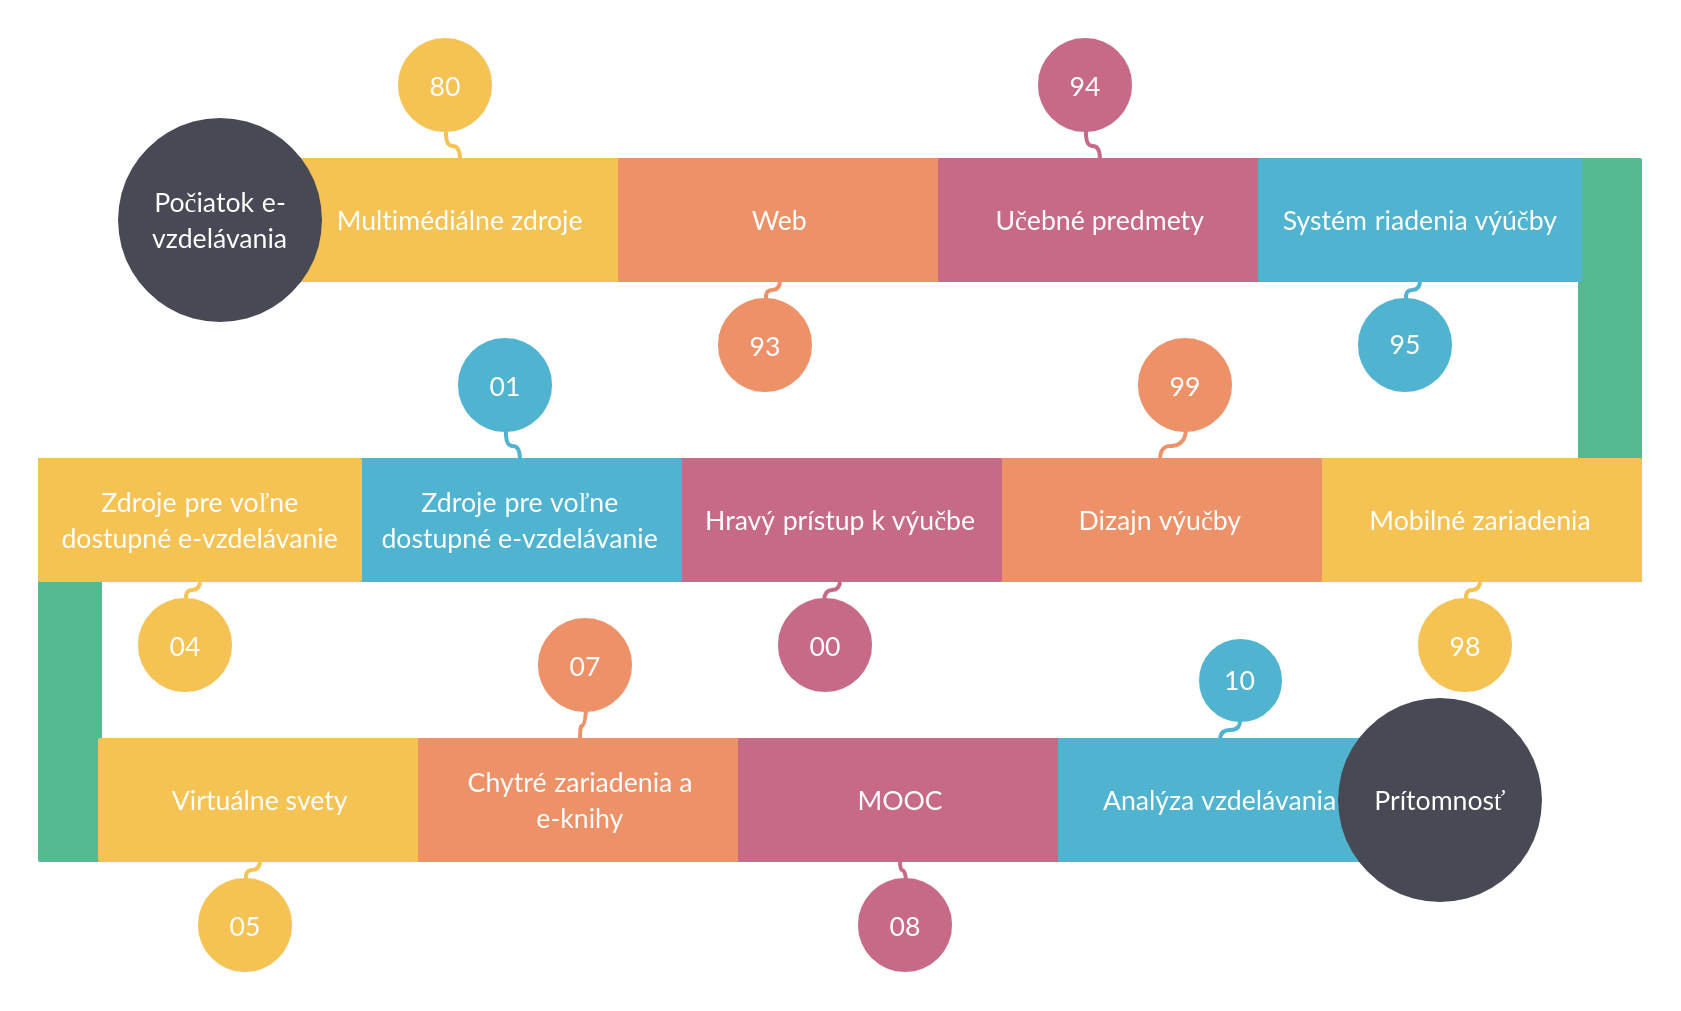
\includegraphics[width = \textwidth]{Obrazky/diagram.png}
		\caption{Rozvoj e-vzdelávania}
		\label{obrazok-casovyDiag}
		\cite{conole}
	\end{figure}

	\subsection{Prvá generácia}
	Prvá generácia je charakterizovaná vznikom online platform na výučbu a to práve vďaka vzniku webu a nápadov vyučovať žiakov prostredníctvom osobných počítačov. V tejto generácií je upriamená pozornosť najmä na obsah výučby a technologické problémy a pedagogické problémy online výučby sú viac menej prehliadané.
	\cite{main}

	\subsection{Druhá generácia}
	Druhá generácia kladie dôraz najmä na ľudský faktor. Komunikácia a interakcia medzi učiteľom a študentom je veľmi dôležitá pre kvalitnú edukáciu študentov. Druhá generácia sa taktiež snaží ísť na rámec jednoduchého publikovania informácií na web. Wbe 2.0, mobilné technológie a voľné šírenie informácii taktiež výrazne pomohli tejto generácii e-vzdelávania rásť.
	\cite{main}
	
	\subsection{Tretia generácia}
	Tretiu generáciu symbolizuje technologický aspekt. Koncept systéma riadenia výučby sa stáva čím ďalej, tým viac populárnym. Od vzniku webu 2.0 a sociálnych nástrojov sa platforma e-vzdelávania stala súčasťou technologického ekosystému orientovanom na proces výučby. Do systému e-vzdelávania sa ako ľudia zapájame ako úmyselne, tak aj neúmyselne. Preto je možné nájsť určité črty e-vzdelávania aj v klasickom vzdelávaní prezenčnou formou.

	Samozrejme existujú aj iné experimentálnejšie implementácie e-vzdelávania ako napríklad “flipped teaching” (prevrátená výučba) \cite{baker}\cite{lage}.
	V takomto prístupe sa vzdelávanie čo by sa za normálnych okolností dialo doma (napríklad písanie domácich úloh) sa deje v škole a prednes novej témy sa deje keď sú žiaci doma. Taktiež boli pokusy o iné metódy ako samovolný časový manažment vzdelávania alebo využitie voľného času na vzdelávanie. Tieto modely boli zavedené kvôli zvýšeniu interakcie medzi učiteľom a študentom a rozvoju zodpovednosti k vzdelávaniu použitím rôznych virtuálnych nástrojov. Tieto virtuálne prostredia pomôžu študentovi k väčšej databáze učebných zdrojov.

	Do tejto generácie sa taktiež začleňujú aj MOOC (massive open online courses). Tento systém vzdelávania sa spopularizoval najmä kvôli skúšaniu nových modelov výučby a MOOC je práve derivácia z týchto modelov. Z tohto štýlu výučby sa časom odvodilo viac podobných konceptov ako napríklad skill MOOC, transfer MOOC, connectivisMOOC...
	\cite{main}
\section{Pedagogické postupy v e-vzdelávaní} \label{pedagogicalApproaches}
	V predošlej sekcii sme sa pozreli na evolúciu e-vzdelávania a na určité postupy vzdelávania. V tejto sekcii sa budeme zameriavať na evolúciu e-vzdelávania s prihliadnutím na pedagogický postup.

	Pedagogické prístupy sú odvodené od teórií učenia, ktoré poskytujú všeobecné informácie
zásady pre navrhovanie konkrétnych stratégií výučby a učenia. Sú mechanizmom na prepojenie teórie s praxou. Dizajnéri pedagogických stratégií vytvárajú stratégie pre učiteľov, ktoré uľahčujú výučbu študentov. Podľa Dabbaghovej existujú tri kľučové prvky, ktoré podporujú zmysluplné učenie a interakciu\cite{dabbagh}:
	\begin{itemize}
		\item Pedagogické modely
		\item Inštruktáže a vzdelávacie stratégie
		\item Pedagogické nástroje alebo online vzdelávacie technológie
	\end{itemize}
	Tieto tri komponenty tvoria stály vzťah, v ktorom pedagogické modely informujú o koncepcii e-vzdelávania vedením k špecifikácií učebných stratégií, ktoré sú následne umožnené alebo uskutočnené pomocou využitia technológií na výučbu. Vzhľadom na skutočnosť, že učebné technolúgie sa stali všadeprítomnými a stále pribúda mnoho nových technológií, pedagogické postupy sa stále vyvíjajú a menia, to ale neznamená, že pôvodné pedagogické postupy vymiznú, práve naopak, ako bolo spomínané vyššie, generácie e-vzdelávania nezmiznú, ale koexistujú. Napríklad niektoré modely sa stále používajú, ale len sú obohatené o nové stratégie, ako napríklad gamifikácia. 
	\cite{main}

	Profesorka D.Conole rozdelila pedagogické postupy e-vzdelávania do štyroch kategórií\cite{conoleBook}:

	\begin{figure}
		\centering
		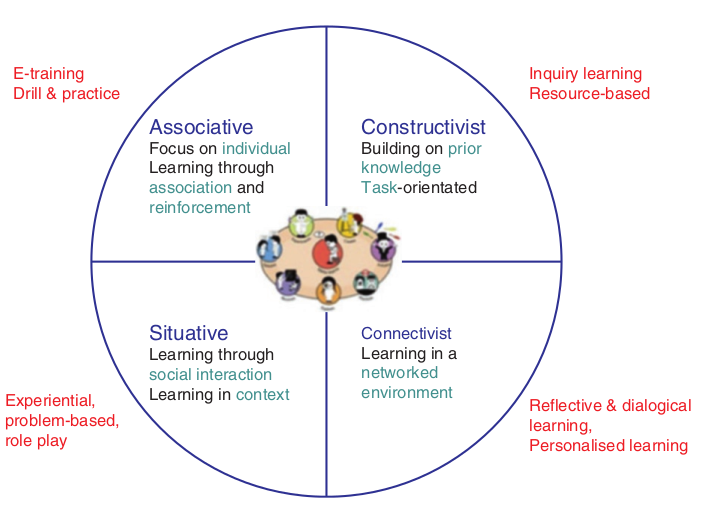
\includegraphics[width = \textwidth]{Obrazky/Pedagogicke postupy.png}
		\caption{Pedagogické postupy e-vzdelávania}
		\label{obrazok-pedagPostupy}
		\cite{pedagPostupy}
	\end{figure}
	
	\begin{enumerate}
		\item Asociatívne vzdelávanie - tradičná forma vyučovania, dôraz je kladený najmä na výučbu teoretických informácií pomocou klasického prednesu učiva a rôznych cvičení.
		\item Kognitívne / konštruktivistické vzdelávanie - hlavnou úlohou je spracovanie a porozumenie nových informácií, ktoré nadväzujú na vedomosti študenta. Zvyčajne sa vyučuje pomocou praktických úloh, čo musí študent robiť.
		\item Situačné vzdelávanie - vyučovanie na základe sociálnej interakcie študenta, každý študent má zodpovednosť sám za seba, že čo sa naučí. Tento štýl je preto chápaný ako zameraný na žiaka.
		\item Konektivistické vzdelávanie - výučba po sieti. Tento štýl výučby počíta s tým, že sa študent naučí byť viac organizovaný a tým pádom aby bol aj efektívnejší vo výučbe. 
	\end{enumerate}

	Vývoj prvých platform určených na e-vzdelávanie bol založený na asiciatívnom vzdelávaní. Proces návrhu tento výučby nasleduje postupná a lineárna štruktúra riadená vopred stanovenými cieľmi a dizajnér predpokladá, že študent je schopný sa všetko naučiť za určité obdobie. Návrhár zoradí učivo od najjednoduchších problémov po tie najzložitejšie, pričom tieto problémy zvyčajne sa seba nadväzujú. Podobný systém sa využíva aj v slovenskom školstve, učiteľ na začiatku roka vypracuje osnovu výučby a žiaci by mali byť schopní sa naučiť určité množstvo informácií a následne ich vedieť aplikovať. Vzhľadom na technologické možnosti dnešnej doby je tento prístup pri online výučbe obmedzujúci, lebo neplánuje praktickú časť výučby, ktorá pri e-vzdelávaní podporuje študenta vo vzdelávaní a dáva mu väčšiu kontrolu nad  celým procesom výučby.
	\cite{main}

	Výber správneho pedagogického postupu sa samozrejme odvíja od toho, čo chceme docieliť, ale ešte dôležitejšie je uvedomiť si rozdiel medzi návrhom plánu pre prezenčné a dištančné vzdelávanie.
	\cite{main}

	Výskumy zaoberajúce sa e-vzdelávaním sa zhodujú na fakte, že jedným z najvýznamnejších pre kvalitné e-vzdelávanie je kvalitný návrh online kurzov tak, aby sa v nich vyskytoval kontent, ktorý zabezpečí interakciu študenta s učiteľom, študenta so spolužiakmi a flexibilnejšie dátumy odovzdania projektov, aby si študent mohol zvoliť správne tempo, ktoré práve jemu vyhovuje v online vzdelávaní.
	\cite{main}
%\section{Ekosystémy vzdelávania} \label{ecosystems}

\section{Reakcia ne témy z prednášok} \label{reakcia}
	\paragraph{Spoločenské súvislosti.}

	V dnešnej dobe využívame technológie prakticky všade. Na spoločnosť je určitý tlak, aby každý vedel aspoň základne obsluhovať počítač. Úlohou nás, informatikov, je zlepšovať informačné systémy tak, aby ľudia, čo ich využívajú v ich odvetví mohli čo najviac venovať svojej robote. 

	\paragraph{Historické súvislosti.}

	Znalosť histórie svojho obora je užitočná na pochopenie určítých súvislostí. História informačných technológií nám pomáha hlbšie pochopiť ako a prečo vznikali rôzne algoritmy, architektúry, programovacie jazyky a podobne.

	\paragraph{Technológia a ľudia.}

	Vývoj nových technológií a využívanie existujúcich technológií ľuďom zjednodušuje život. Hoci niekedy prechod z klasickej formy uchovávania údajov vie byť zdĺhavý a zdanlivo obtiažny proces, s rozostupom času väčšina ľudí zistí, že spravovanie dát je vďaka technológiám jednoduchšie.



\section{Záver} \label{zaver} 
% týmto sa generuje zoznam literatúry z obsahu súboru literatura.bib podľa toho, na čo sa v článku odkazujete
\bibliography{literatura}
\bibliographystyle{plain} % prípadne alpha, abbrv alebo hociktorý iný
\end{document}
